% !TEX TS-program = pdflatex
% !TEX encoding = UTF-8 Unicode

% This is a simple template for a LaTeX document using the "article" class.
% See "book", "report", "letter" for other types of document.

\documentclass{allertonproc} 

%%% Examples of Article customizations
% These packages are optional, depending whether you want the features they provide.
% See the LaTeX Companion or other references for full information.
\usepackage{cite}
\usepackage{graphicx} % support the \includegraphics command and options
\usepackage{amsmath}
% \usepackage[parfill]{parskip} % Activate to begin paragraphs with an empty line rather than an indent
\usepackage{placeins}
%%% PACKAGES
\usepackage{booktabs} % for much better looking tables
\usepackage{array} % for better arrays (eg matrices) in maths
\usepackage{paralist} % very flexible & customisable lists (eg. enumerate/itemize, etc.)
\usepackage{verbatim} % adds environment for commenting out blocks of text & for better verbatim
\usepackage{subfig} % make it possible to include more than one captioned figure/table in a single float
% These packages are all incorporated in the memoir class to one degree or another...

\renewcommand{\topfraction}{0.85} 
\renewcommand{\bottomfraction}{0.85} 
\renewcommand{\floatpagefraction}{0.8}
%%% The "real" document content comes below...

\title{SPATIAL CHANNEL PREDICTION FOR EAVESDROPPING ON WIRELESS FADING BASED KEY GENERATION} %this title is not bad
\author{Eric Brown, Clara Gamboa, and K.~C.~Kerby-Patel\\University of Massachusetts Boston, Boston, MA\\kc.kerby-patel@umb.edu} %the convention is that the advisor's name goes last
%also have to put in our UMB affiliation blurb
\date{} % Activate to display a given date or no date (if empty),
         % otherwise the current date is printed 

\begin{document}
\maketitle
\bibliographystyle{ieeetran}

\begin{abstract}

Physical layer key generation techniques based on wireless channel fading are generally considered to be secure as long as any eavesdroppers are separated from the terminals by a distance greater than the channel correlation length.  In fact, this is true only if the channel observations are jointly Gaussian random variables, which is often not the case in real channels.  A channel's transfer function is determined by the physical scatterers in that particular channel realization, and information about the legitimate nodes' channel may persist over significantly longer distances than the correlation length if the physical parameters of the channel are slowly varying.  Linear prediction has previously been employed to predict samples of the channel transfer function ahead in time.  In this work, we demonstrate that it is also possible to predict the channel transfer function ahead in space, over distances larger than the correlation length.  This leads to the conclusion that a more pessimistic minimum safe eavesdropper distance for link signature keying is needed.
\end{abstract}
%we will have to compute the correlation length from the observed channel covariance matrix.  

%\textbf{Key words:} -- wireless, channel, fading, key generation, physical layer, security

\section{Introduction}
It has been demonstrated \cite{azimisadjadi2007, bloch2008, mathur2008, ye2010} that two parties' reciprocal observations of a fading wireless channel can be used as a common source of randomness to generate symmetric encryption keys in cases where two parties cannot pre-arrange or securely exchange keys.  Each party transmits a predetermined waveform, which the other party receives and uses to determine the channel transfer function.  These measurements are assumed to be the same in both directions if completed within a short period of time, because of the channel's reciprocity.  This technique has been referred to by a number of names, including fading-based key generation and link signature keying.  Since the channel transfer function is also position dependent, eavesdroppers at other locations observe a different channel transfer function and the legitimate nodes' channel measurements are usually assumed to be secret.  In order for this technique to be useful as a practical encryption method, the secrecy of the channel measurements must be quantified.  This work examines how, and under what circumstances, an eavesdropper could predict the channel observations of the communicating parties.

The security claim of link signature keying is based on the assumption that if an eavesdropper is located farther than a correlation length from the communicating parties, it will have essentially no information about the symmetric key generated from their reciprocal channel measurements \cite{azimisadjadi2007, bloch2008, mathur2008, ye2010, he2013}.  Since the channel correlation function in many channels falls off quickly with distance \cite{jakes1974}, the minimum secure distance is often stated to be a half wavelength.  However, mutual information between two channel observation locations may be high even if the channel correlation function is low or has a minimum, since the channel transfer function is a deterministic function of physical environmental parameters such as the amplitudes and phase delays of the scattering paths in the channel.  Although the values of these environmental parameters may be unknown to all parties, they often vary quite slowly with distance compared to the correlation function of the channel \cite{jakes1974, duel-hallen2007}.  The mutual information between the channel parameters at two locations represents an upper bound on the mutual information between channel observations at those locations \cite{kckpVTC2015}.  Such information may persist over distances longer than the correlation length, so security claims based on the correlation length are inappropriate.  In this work, we apply channel prediction techniques \cite{duel-hallen2007} to investigate the distance over which it is possible to predict the channel transfer function.

A similar but narrower problem was identified by He \emph{et al}.~in \cite{he2013}.  That work pointed out that the correlation functions of some channels have broad peaks in the spatial domain, and link signature keying using such channels is vulnerable to correlation-based attacks based on linear minimum mean-square error estimation.  By contrast, the minimum secure distance discussion we present is not based on the width of the correlation function but on the mutual information between separated channel observations, which can persist even when the correlation function is highly oscillatory and has a narrow peak.  As a result, it applies to a more general set of channels and is not limited to those with low angular spread.  In order to predict a channel with wide angular spread, the eavesdropper in this work is assumed to use a parameter estimation technique.

Section \ref{mutualinfo} briefly summarizes the argument for a mutual information based minimum secure distance that was presented in \cite{kckpVTC2015}.  Next, Section \ref{prediction} outlines a method by which an eavesdropper may apply long-range prediction techniques to a series of spatial samples in order to predict the channel transfer function over distances greater than the correlation length.  In Section \ref{simresults}, this technique is applied to a simple simulated channel to examine the dependence of prediction length on the properties of the channel and the eavesdropper array. 

\section{Mutual Information vs.~Correlation}\label{mutualinfo} %this needs a better section heading?
The ability of an eavesdropper to estimate the legitimate nodes' encryption key depends on the mutual information between the eavesdropper's channel observations and the legitimate nodes' observations.  In the literature, the channel correlation function is usually used as a proxy for the mutual information.  In \cite{kckpVTC2015} it was argued that this leads to an inappropriately optimistic minimum secure eavesdropper distance, and an eavesdropper may be able to predict the legitimate nodes' channel observations despite being more than a correlation length away.  This section briefly summarizes that argument, which is the motivation for the channel prediction simulation that follows.

If two random variables are jointly Gaussian, their mutual information is a monotonic function of their correlation function.  Thus, jointly Gaussian observations of a wireless channel at two locations, $h(\mathbf{r})$ and $h(\mathbf{r}+\mathbf{\Delta r})$, have mutual information given by 
\begin{equation}\label{mutualinformationgauss}
I(h(\mathbf{r}),h(\mathbf{r}+\mathbf{\Delta r})) = -\frac{1}{2}\ln\left(1-\frac{R_h(\mathbf{r},\mathbf{r}+\mathbf{\Delta r})}{\sigma_h^2}\right)
\end{equation}
where $R_h$ is the correlation function, defined as usual, and $\sigma_h^2$ is the average power.
\begin{equation}
R_h(\mathbf{r},\mathbf{r}+\mathbf{\Delta r}) = E[h(\mathbf{r})h^*(\mathbf{r}+\mathbf{\Delta r})]
\end{equation}

If the two observations are not jointly Gaussian, the expression given in (\ref{mutualinformationgauss}) is merely a lower bound on the mutual information.  In general, the channel transfer function at a particular location is a deterministic function of a set of environmental parameters $\boldsymbol{\theta}$ at that location. The environmental parameters may be considered to be a random variable. The data processing inequality can be applied to find that the mutual information of channel transfer function values at two locations with environmental parameters $\boldsymbol{\theta_1}$ and $\boldsymbol{\theta_2}$ is bounded by the mutual information of the environmental parameters.
\begin{equation}\label{ineq1}
I(h(\boldsymbol{\theta_1},\mathbf{r_1}); h(\boldsymbol{\theta_2},\mathbf{r_2}))\leq I(\boldsymbol{\theta_1}; \boldsymbol{\theta_2})
\end{equation}

Observations of the channel are given by $\tilde{h}(\boldsymbol{\theta})=h(\boldsymbol{\theta})+n$, where $n$ is additive white Gaussian noise.  The mutual information between two observations is limited by the mutual information between the channel transfer function itself at those two locations, again by the data processing inequality.  Equation (\ref{ineq2}) is further bounded by (\ref{ineq1}).
\begin{equation}\label{ineq2}
I(\tilde{h}(\boldsymbol{\theta_1},\mathbf{r_1}); \tilde{h}(\boldsymbol{\theta_2},\mathbf{r_2}))\leq I(h(\boldsymbol{\theta_1},\mathbf{r_1}); h(\boldsymbol{\theta_2},\mathbf{r_2}))
\end{equation}

If the observations are close enough to each other spatially that the environmental parameter vector $\boldsymbol{\theta}$ does not change appreciably, the upper bound on the mutual information between two observations is the entropy of $\boldsymbol{\theta}$.  This means that the two observations may both contain all of the information about the channel parameters.
\begin{equation}
I(\tilde{h}(\boldsymbol{\theta},\mathbf{r_1}); \tilde{h}(\boldsymbol{\theta},\mathbf{r_2}))\leq H(\boldsymbol{\theta})
\end{equation}

This discussion has provided a lower bound and an upper bound on the mutual information between two observations of a wireless channel.  Clearly, significant room remains for variation between the two bounds.  However, it has been observed that environmental parameters are slowly varying spatially compared to the channel transfer function and its correlation function \cite{jakes1974, duel-hallen2007}.  This indicates that information about the legitimate nodes' channel may be available to the eavesdropper even at a distance of more than a correlation length.   The correlation length merely indicates that the value of the correlation function is zero at a particular location and does not necessarily predict the availability of information to an eavesdropper. 

\section{Spatial Long-Range Channel Prediction Method}\label{prediction}
%belongs to Eric
As discussed in Section \ref{mutualinfo}, channel information may persist over distances greater than the correlation length. Therefore, long-range prediction techniques as in \cite{duel-hallen2007} may be applied to predict the channel from spatial samples. Rather than using long-range prediction to predict the channel transfer function ahead temporally, as is the typical usage, this simulation will use spatial sampling and spectral estimation to discover the channel's parameters and reconstruct its transfer function at a distance.

%I feel like this is jsut restating the same thing two different ways

It is assumed that the eavesdropper has knowledge of the location of one of the legitimate nodes, and has the ability to take a number of spatial samples along a line in the direction of that node.  Previous literature has shown that spectral estimation can be applied to a temporal prediction scenario by estimating channel parameters in an assumed channel model, then predicting the channel using the estimated parameters \cite{duel-hallen2007}. In experimental implementation with real-world channels, the channel parameters varied slowly enough that this prediction method was accurate within a Doppler wavelength. In this work a prediction length of a few carrier wavelengths---significantly less than a Doppler wavelength---would be sufficient to demonstrate the inadequacy of the half-wavelength minimum safe distance. Therefore, it is reasonable for the eavesdropper to reconstruct the channel with parameter estimation using spatial sampling and spectral estimation. 

%In temporal prediction applications, it has been observed that time variation of the amplitudes and frequencies in the sum-of-sinusoids model is on the order of 0.1 seconds \cite{duel-hallen2007}. 

\begin{figure}[tbp]
\begin{center}
\includegraphics[height=3in]{Scenario}
\caption{Depiction of an outdoor environment with two transmitters (Alice and Bob) and an eavesdropper (Eve).}\label{scene}
\end{center}
\end{figure}

An example scenario is shown in Figure \ref{scene}. Alice and Bob are both transceivers. Eve is a passive eavesdropper sampling array in line with Bob. Scatterers are represented by the objects surrounding Alice and Bob. It has been observed that most real world channels contain less than 10 significant scattering paths \cite{duel-hallen2000}. 

In the simulation of Section \ref{simresults}, it is assumed that the sender Alice and all the scatterers reside in the far field of the eavesdropper array as well as the desired estimation location. The eavesdropper uses direction of arrival techniques to estimate the amplitudes and spatial frequencies of the scattering paths. Once the eavesdropper estimates the channel parameters, it uses them to reconstruct the channel transfer function. The eavesdropper uses a sampling array of length $Md$, where $d$ is the spacing between measurements and $M$ is the number of spatial samples. The eavesdropper attempts to reconstruct the channel out to a length of $(M+q)d$, where $q$ is number of additional samples between the end of the sampling array and Bob. 

Equation \ref{chan} describes the channel transfer function along the line of eavesdropper samples.
\begin{equation}\label{chan}
h_m= \sum_{n=1}^N \alpha_n e^{-j(k_n)md}
\end{equation}
Above, $h_m$ is the channel transfer function at the $m^{\mathrm{th}}$ location, $N$ is the number of scatterers, $\alpha_n$ is the $n^{\mathrm{th}}$ complex amplitude, and $k_n$ is the spatial frequency of that scatterer along the sampling array.  

The solution to the parameter estimation problem can be broken into two parts: estimating the wave numbers $k_n$, then estimating the complex amplitudes $\alpha_n$. The simulated eavesdropper uses the rootMUSIC algorithm supplied in MATLAB to determine the spatial frequencies of the scattering paths \cite{matlab}. RootMUSIC uses eigenvalue analysis of the channel's correlation matrix to estimate the signal's frequency content. The specific command used in this simulation takes the sampling results, a threshold value, and a maximum dimension value. The threshold value serves to separate the noise subspace from the signal subspace, while the maximum dimension value sets a number of sinusoids that make up the signal supplied. It then estimates the discrete frequency spectrum, as well as providing the signal power of each frequency component. 

In order to determine the complex amplitudes of the scattering paths, the method described in \cite{andersen1999} was used. The spectral estimation algorithm determines the spatial frequency of each scattering path. Constant spatial sampling is used, so (\ref{chan}) is simplified by substituting the signal poles $z_n$ for the complex exponentials.
\begin{equation}\label{complexamp}
h_m = \sum_{n=1}^N \alpha_n e^{-j(k_n)md} = \sum_{n=1}^N \alpha_n z_n^m
\end{equation}

Based on the estimated values of the signal poles, the complex amplitudes can be derived by solving the following linear equations. $\boldsymbol{A}$ is a Vandermonde matrix of signal poles, where the $M^\mathrm{th}$ row contains all the poles raised to the $(M-1)^\mathrm{th}$ power. 
\begin{equation}\label{matrix}
\mathbf{h} = \mathbf{A \boldsymbol{\alpha}}
\end{equation}

Equation \ref{matrix} is a system of linear equations of complex amplitude $\boldsymbol{\alpha^T} = [\alpha_1, \alpha_2,... ,\alpha_M]$. The estimated complex amplitudes $\boldsymbol{\hat{\alpha}}$ are then found by solving (\ref{matrix}) for $\boldsymbol{\alpha}$ \cite{andersen1999}.
\begin{equation}\label{ahat}
\boldsymbol{\hat{\alpha}}=\boldsymbol{(A^HA)^{-1}A^Hh}
\end{equation}



%direction of arrival applications typically take many snapshots of

The weakness of using spectral estimation, and rootMUSIC in particular, is the sensitivity to noise in the signal. Direction of arrival applications typically take many snapshots over a span of time and average them to mitigate noise. The simulated eavesdropper is assumed to use this same procedure. The result is an effective signal-to-noise ratio (SNR) increase by a factor of the number of averaged snapshots. 



\section{Spatial Long-Range Channel Prediction Simulated Results}\label{simresults}
%Should we take a baseline average prediction length at default values?

Section \ref{prediction} described a plausible channel estimation process for a hypothetical eavesdropper. In this section, a Monte Carlo simulation is used to determine the average maximum estimation distance for the scenario with varying channel parameters. Each value of each variable which shows impact on the estimation outcome is simulated in 1000 randomly generated channel scenarios. An average is assembled for each swept variable in the Monte Carlo. During each of the 1000 runs, the first sample number at which the difference between the estimate and the true channel exceeds 5\% of the root-mean-square amplitude of $h$ is recorded.  This sample number is the maximum estimation distance.  Plots in this section show the average result after completion of the Monte Carlo simulation for each value of each swept variable.
%edited by KC - I just meant that you should say the error is abs(h-h_hat)/h_rms.
%This error is computed by assembling an array, which is populated for each sweeping variable by taking the max value of each pass, dividing it by the number of runs, then adding it to the value of that array position. 
  %insert graphs and refer to them 

%I changed the letter associations for agreement with earlier math.
The Monte Carlo simulation tests 7 different variables: $M$, the number of samples taken; $d$, the sample spacing in terms of wavelength; $N$, the number of scatterers; $O$, the number of observation snapshots; $P$, the maximum number of sinusoids allowed in the rootMUSIC estimate; $T$, the threshold value used in the rootMUSIC algorithm to separate the signal and noise subspaces; and SNR, the signal-to-noise ratio.

Each parameter is swept over a reasonable span to determine the estimation's sensitivity to that parameter, with all other parameters held constant in a default scenario. The resultant average sample values are plotted against each swept parameter. The Cram\'er-Rao lower bound presented in \cite{kckpVTC2015} was used to identify suitable parameters for a default simulation scenario. These parameters are: $M = 133$; $d = .3$; $N = 7$; $O = 100$; $P = 33$; $T = 100$; SNR $= 13$dB. The array length in carrier wavelengths with these parameters is $40\lambda$ and the averaging raises the effective default SNR to $33$dB. For reference, a 1000 iteration Monte Carlo simulation was conducted using the default scenario.The average maximum prediction length past the sampling array was $21\lambda$.

%%%REFER TO VTC PAPER: "The CRLB expressions presented in \cite{**vtc**} were used to identify suitable parameters for a default simulation scenario.   ...more details and maybe graphs if we feel like it.  Putting this in its own subsection might be a good idea.

%How do I introduce the defaults of the scenario without explaining line by line what the code is?
\begin{figure}[tbp]
\begin{center}
\includegraphics[width=6in]{numMeasurements}
\caption{Plot showing the increase of samples and array length improving the estimation quality, then deteriorating slightly past 300 samples. $d = 0.3\lambda$ is the default spacing interval}\label{M}
\end{center}
\end{figure}
Figure \ref{M} shows the number of samples in the eavesdropper's sampling array. It is evident that the quality of the estimation increases significantly up to 160 samples, then levels off. With the default spacing of $d = 0.3\lambda$, a measurement length of 160 samples corresponds to 48$\lambda$. The average maximum prediction length with 160 samples is 130 samples past the sampling array, or 39$\lambda$.
%insert figure 1

\begin{figure}[tbp]
\begin{center}
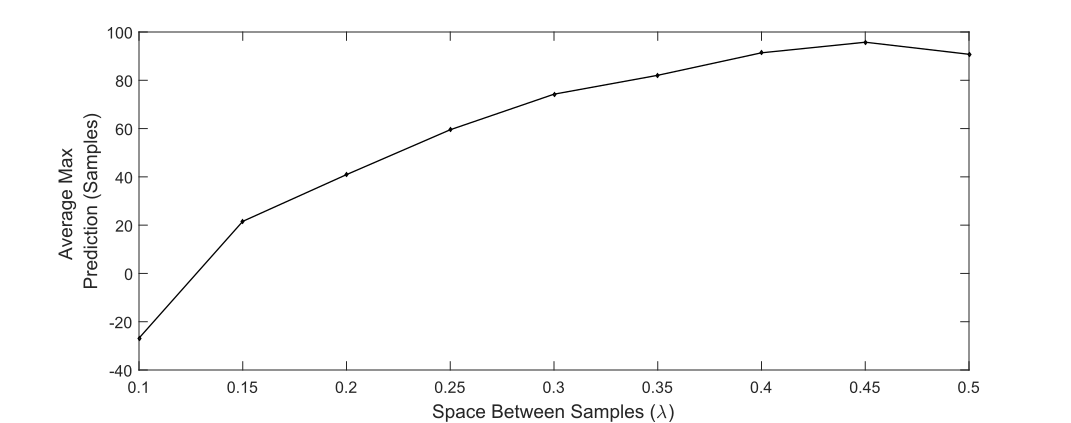
\includegraphics[width=6in]{wavelengths}
\caption{Average maximum prediction length vs. the spacing between samples. The default number of samples in the eavesdropper array in this test is $M = 133$.}\label{spacing}
\end{center}
\end{figure}
Figure \ref{spacing} shows the average maximum prediction length vs. the spacing between spatial samples. There is a steady increase in the estimation quality of the array as the spacing increases. The number of samples remains constant as the spacing is increased, so the length of the array grows throughout the test. At the spacing of 0.45$\lambda$ the length of the eavesdropper array is approximately 60$\lambda$, with the resulting maximum prediction length being 43$\lambda$. Further testing has shown that the estimation quality levels out at $0.45\lambda$.
%insert fig 2

\begin{figure}[tbp]
\begin{center}
\includegraphics[width=6in]{numScatterers}
\caption{Average maximum prediction length vs. the number of scatterers.}\label{Scatter}
\end{center}
\end{figure}
Figure \ref{Scatter} shows how the average maximum prediction length varies depending on the number of scatterers in the scenario. Predictably, additional scattering paths increase the complexity of the estimation problem. With this eavesdropper configuration, there is a smooth drop-off in the quality of the estimation, finally failing to predict past the sampling array at 10 scatterers. This is consistent with the behavior predicted in \cite{kckpVTC2015}. Changing aspects of the eavesdropper configuration, such as averaging more snapshots to further limit the noise of the sampled signal, can improve the prediction capabilities past 10 scatterers.

\begin{figure}[tbp]
\begin{center}
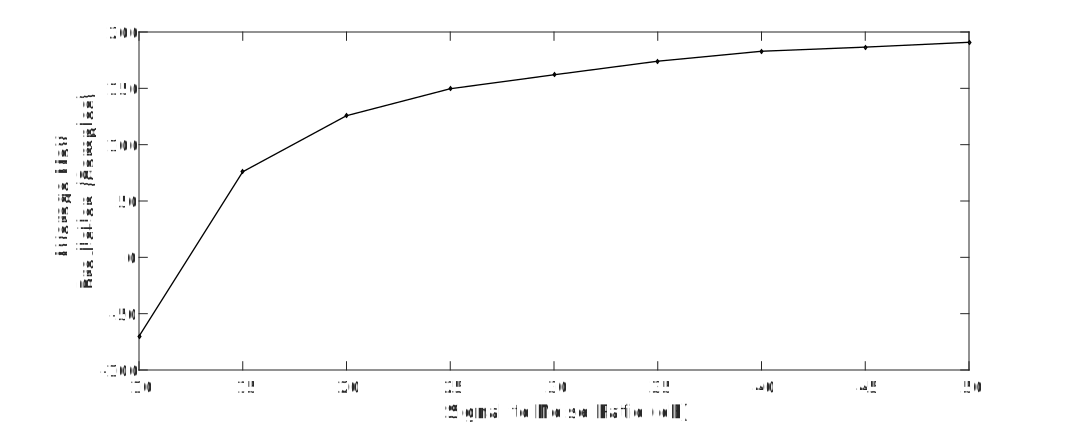
\includegraphics[width=6in]{signalToNoise}
\caption{Average maximum prediction length vs. SNR. }\label{SNR}
\end{center}
\end{figure}
Figure \ref{SNR} shows how increasing the signal-to-noise ratio of the eavesdropper observations greatly increases the estimation performance and extends the average maximum prediction length. The default value for the simulations in all other tests was $13$dB. In all tests, including the swept SNR tests used to generate this plot, the eavesdropper averages 100 snapshots. The averaging produces an additional processing gain of $20$dB. Estimation performance drastically improves at SNR values above $24$dB ($44$dB including the gain due to averaging). Signal-to-noise ratio is the most important factor in the effectiveness of the estimation method.

\begin{figure}[tbp]
\begin{center}
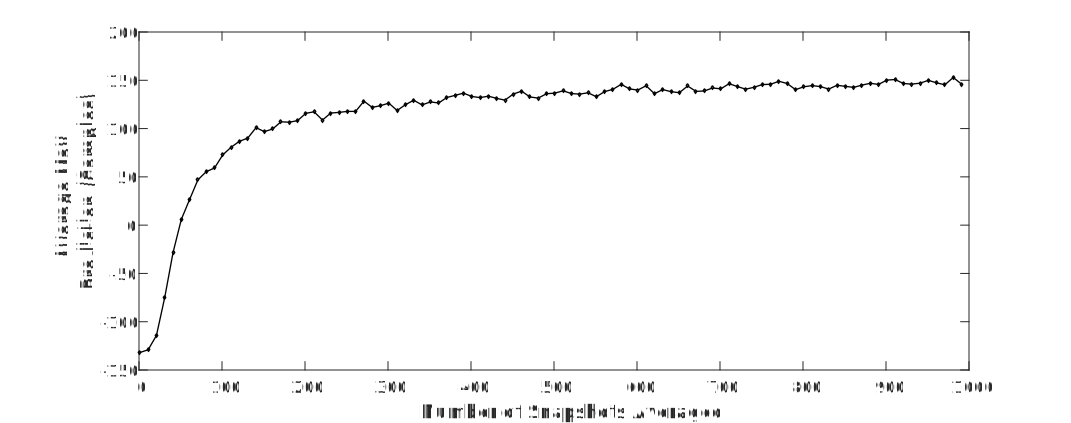
\includegraphics[width=6in]{numSnapshots}
\caption{Average maximum prediction length vs. number of snapshots averaged. At 75 snapshots the estimation reaches the end of the sampling array, and by 100 snapshots the estimation is good enough to predict several wavelengths.}\label{snapshot}
\end{center}
\end{figure}
Figure \ref{snapshot} shows that averaging multiple observation snapshots of the same channel realization has a great impact on signal quality. This figure shows that for the default scenario 100 snapshots is sufficient to significantly improve the performance., raising the effective SNR to $33dB$. Direction of arrival applications typically use 100 to 1000 snapshots, so the usage here is well within the realm of possibility. %bleh

\begin{figure}[ptb]
\begin{center}
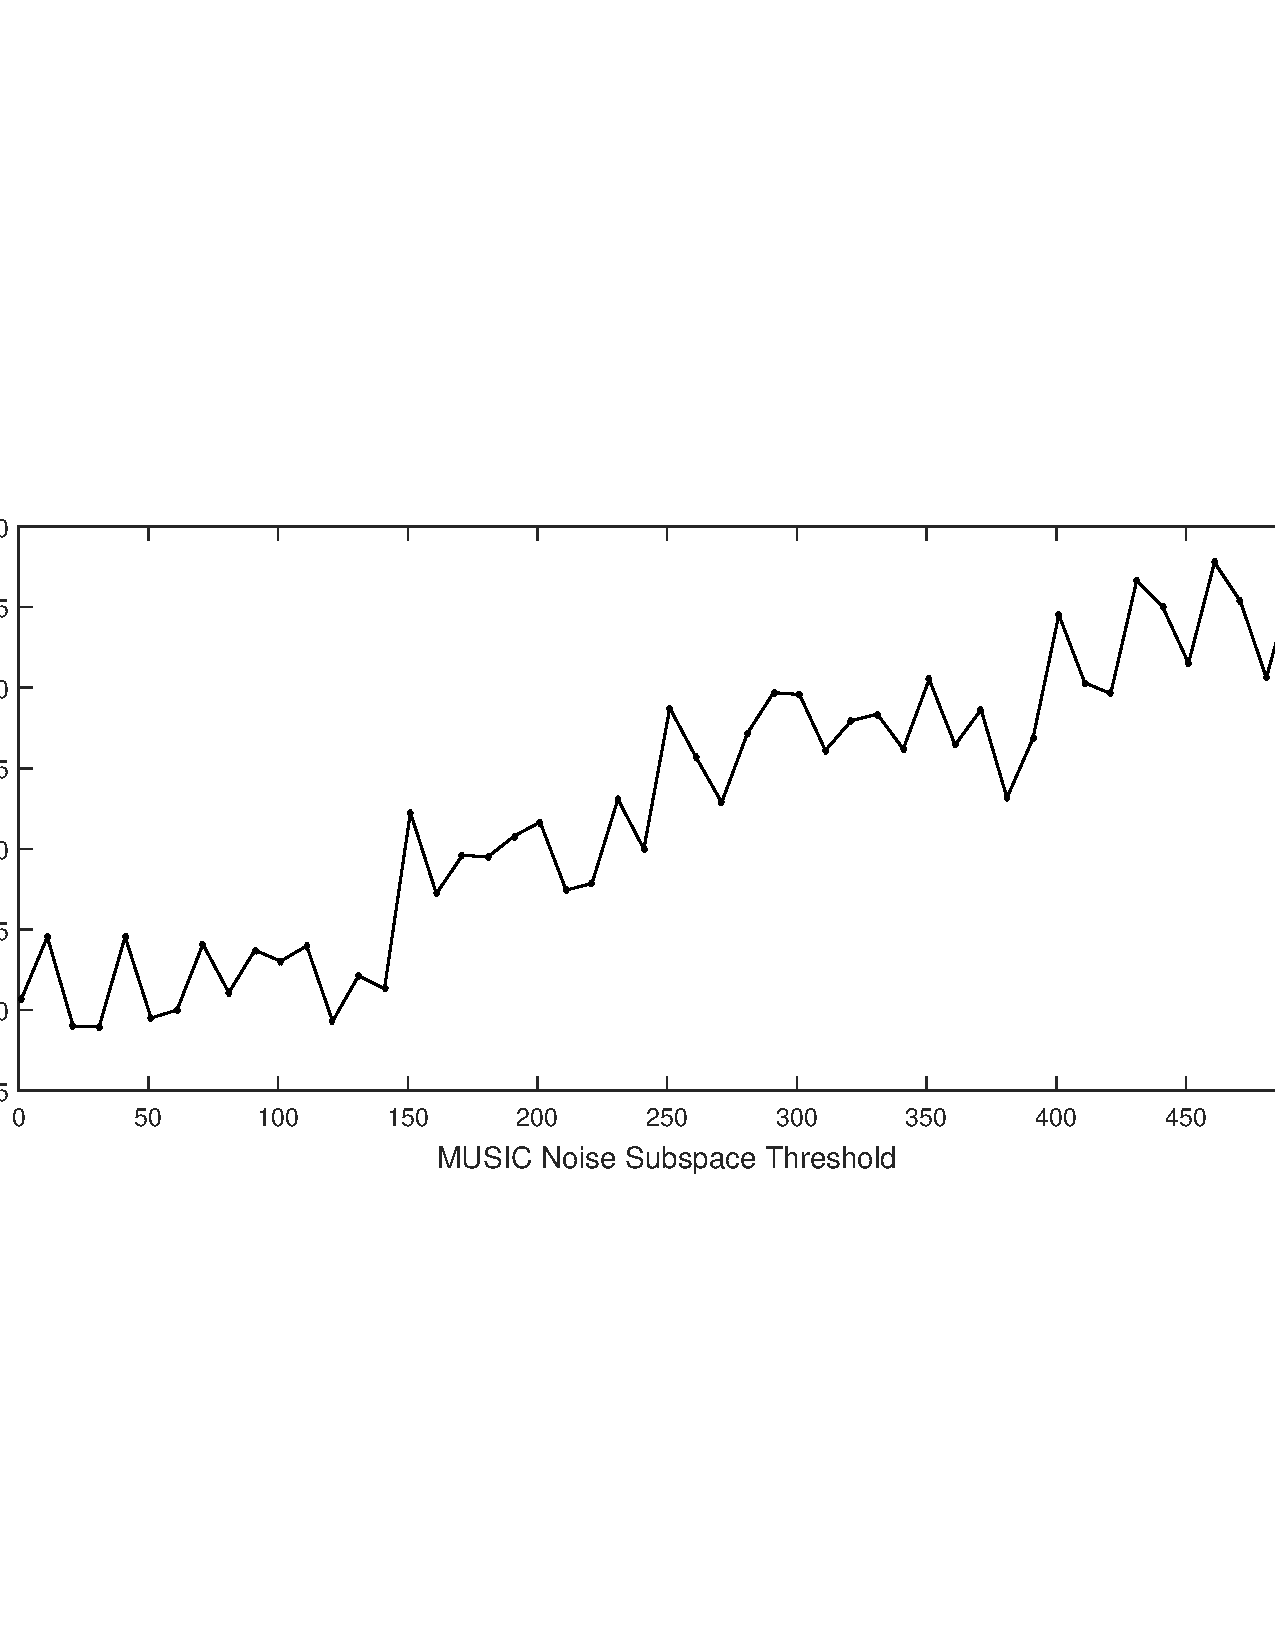
\includegraphics[width=6in]{musicNoise}
\caption{Average maximum prediction length vs. noise subspace threshold. }\label{thresh}
\end{center}
\end{figure}

\begin{figure}[ptb]
\begin{center}
\includegraphics[width=6in]{numSinusoids}
\caption{Average maximum prediction length vs. maximum dimension of the signal subspace. }\label{sinusoid}
\end{center}
\end{figure}
The rootMUSIC algorithm uses the threshold value to separate the signal subspace of the correlation matrix from the noise subspace. Eigenvalues below the smallest estimated eigenvalue of the signal's correlation matrix, $\lambda_{min} *T$ are assigned to the noise subspace\cite{matlab}. Figure \ref{thresh} shows the average maximum prediction length plotted vs. the rootMUSIC modifier threshold. There is a general trend towards better quality of the estimate using higher noise threshold, however the improvement is unpredictable value to value.%I don't really know what to say here. It's spiky, but I don't really know why 

Figure \ref{sinusoid} shows the effect of the second modifier value for the rootMUSIC algorithm. This value specifies the maximum dimension of the signal subspace. For the default scenario, a value of 20 is optimal for prediction length. The threshold modifier, and to a lesser extent the maximum dimension modifier are both very sensitive to changes in the scenario construction. If the sampled correlation matrix is too small or too large vs. these modifier values the performance of the estimation is severely degraded. Additionally, the performance of the threshold value for a given scenario is extremely uneven, as evidenced by the roughness of the plot in Figure \ref{thresh}.

\FloatBarrier
\section{Conclusion}

The simulated results provided here indicate that an eavesdropper could reconstruct the channel transfer function at a particular location from more than a correlation length away by applying long-range prediction to estimate the channel transfer function.  This indicates that the minimum safe distance for secure key generation based on wireless fading must be reexamined.

In order to successfully predict the wireless channel at a distance in the scenario constructed here, the eavesdropper must know details about the environment, specifically the location of Bob. Besides this knowledge, the eavesdropper would have to possess a large sampling array on the order of tens of wavelengths in length, and the processing power to conduct the estimation. The situation for the eavesdropper improves with higher SNR, however using the method of averaging used in the simulation that would only be achieved by higher and higher dwell times. So while possible, estimating a channel in this manner is far from trivial. %what else?

This work invites investigation of a number of additional questions. The immediate next step is to demonstrate the feasibility of spatial channel prediction experimentally.  Future investigations will attempt to identify alternative eavesdropper array geometries and estimation techniques that are more efficient or robust.  Situations in which the scatterers are not in the far field of the eavesdropper may require time difference of arrival analysis techniques rather than spectral estimation.   Thorough understanding of the potential capabilities of an eavesdropper will lead to strategies that the legitimate nodes may implement for improved security.

%our analysis is potentially pessimistic because we assume the channel parameters don't change within the sampling interval - however, it may be possible to extend the estimation to include both the channel parameters and their first derivatives.  CRLB will increase because it usually increases with additional parameters.

%future work: do a scenario where the eavesdropper moves through space and see if we can do spatiotemporal channel prediction simultaneously, see about 2D eavesdropper arrays and other problem geometries (what if all the scatterers are in an arc of the space instead of evenly distributed? does it matter?), do a security analysis by estimating the error of the prediction(?), demonstrate spatial channel prediction experimentally, investigate the effect of mutual coupling between array elements on the quality of the eavesdropper's predictions
\bibliography{PL-Library}{}
\end{document}